\chapter{Figures and Tables}
As you might know already, both figures and tables are considered \glspl{float}. Depending on the discipline/institution, you might need to set up your float in some specific ways. Some people like to anchor floats to the top of the page, so it is easy to find them. When I wrote my thesis, it was preferable to put floats after and closest possible to the first texts that describe them, so I set floats to \texttt{[ht!]}, which forces floats to be either ``here'' or at the ``top'' of the next page, as seen in the figures and tables in this chapter. You can read more about float settings \href{https://www.overleaf.com/learn/latex/Positioning_of_Figures}{here}. In addition, for long tables, it is beneficial to know how \href{https://mirror.aarnet.edu.au/pub/CTAN/macros/latex/contrib/tabulary/tabulary.pdf}{\texttt{tabulary}} works.

\section{Colour choice}

When it comes to colours, make sure you accommodate for colour-blind people. There are two ways to do this: (1) for things like scatter plots and line graphs, use colours in combination with shapes; (2) use colour-blind friendly colour-pallets, like \href{https://cran.r-project.org/web/packages/viridis/vignettes/intro-to-viridis.html}{viridis}, particularly for heatmaps. 

Sometimes you might find yourself wanting to pick a colour that is not predefined by your graphic tools (like red, blue, etc). In that case you might find \href{https://www.w3schools.com/colors/colors_picker.asp}{this site} very helpful, as you can pick a colour and get a universal code for them. You might know this already, but one of the worst combinations of colours possible is red and green, unless you are deliberately sexist against males - \href{https://visioneyeinstitute.com.au/eyematters/colour-blindness/}{8\% of the male population and 0.4\% of the female population is red/green colour blind}.

Finally, \href{https://betterfigures.org/2015/06/23/picking-a-colour-scale-for-scientific-graphics/}{here} are some final tips for good colour choice.

\section{Subfigures and subtables}

It might be often the case that you need to bundle figures or tables or both together into subfigures or subtables to convey information. In that case you will need to use subfigures or subtables. Figure \ref{fig:demo} shows an example of a collection of two figures (Figure \ref{fig:pets}) and \ref{fig:iphone}) and a table (\ref{tab:cats}). For tables only, you might use subtables. (Note that to be able to use subfigures, I put the package \texttt{subcaption} in \texttt{setup.tex}).

\begin{figure}[ht!]

  \begin{subfigure}[c]{0.5\textwidth}
    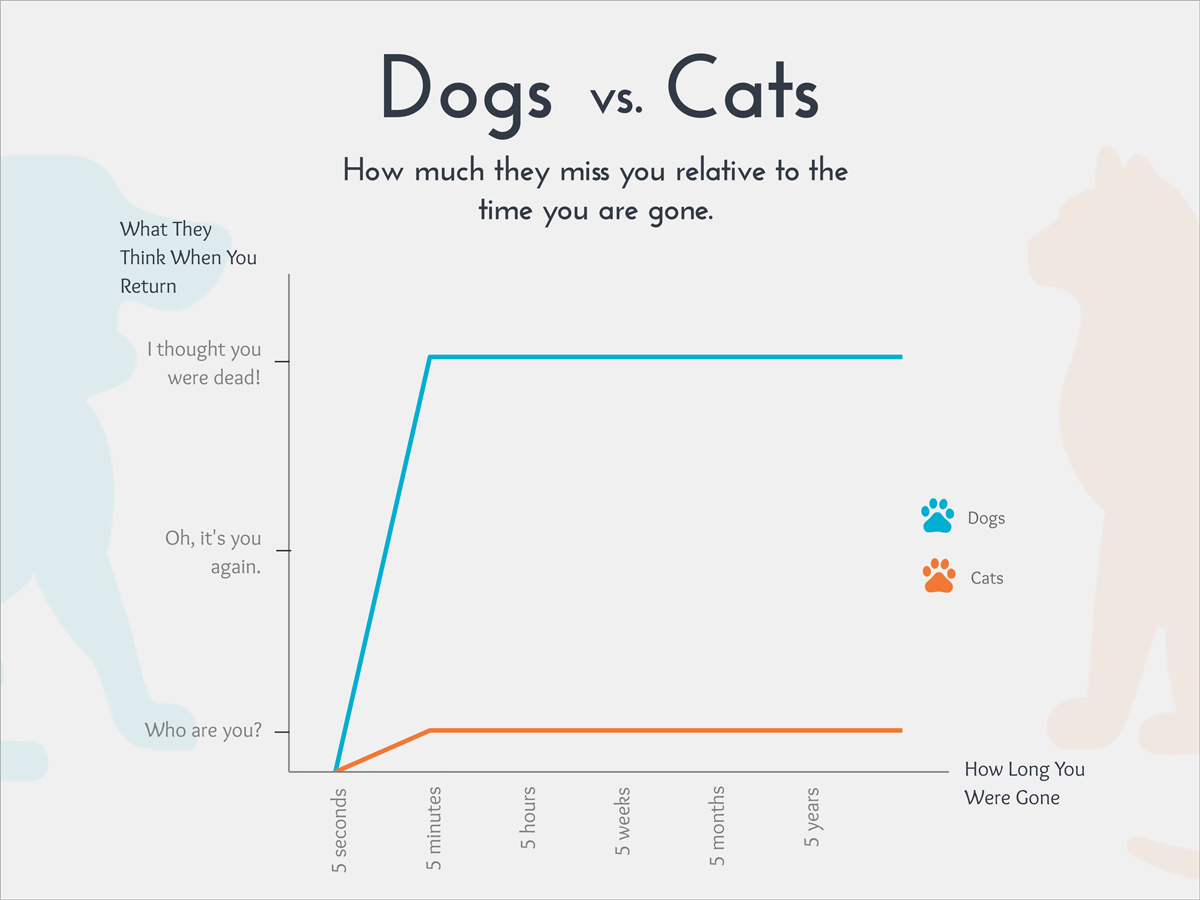
\includegraphics[scale=0.18]{graphics/dogs_vs_cats.png}
    \caption{Dogs \textit{v.s.} cats}
    \label{fig:pets}
  \end{subfigure}
  \vspace{0.3cm}
  ~
  \begin{subfigure}[c]{0.5\textwidth}
    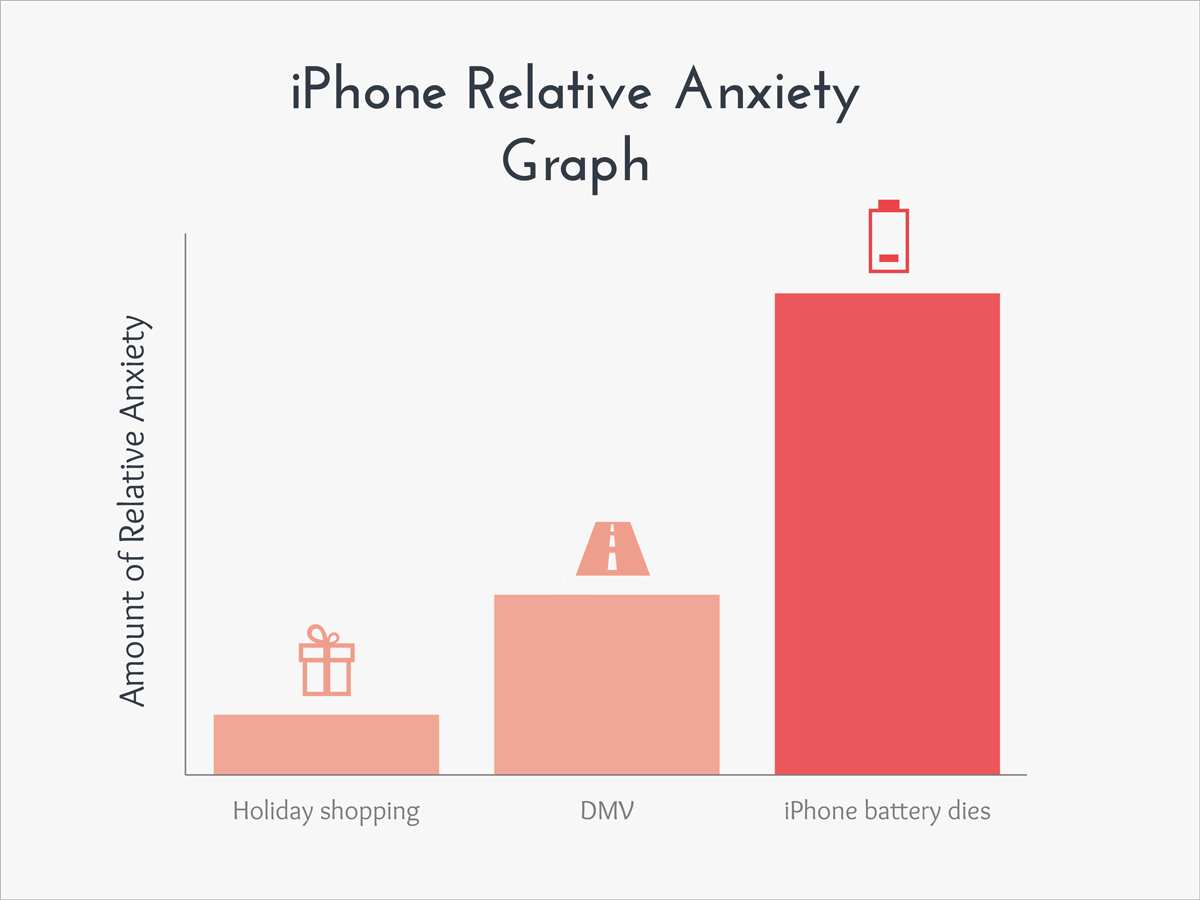
\includegraphics[scale=0.18]{graphics/iphone.png}
    \caption{iPhone anxiety}
    \label{fig:iphone}
  \end{subfigure}
  \vspace{0.3cm}
  
  \begin{subfigure}[c]{\textwidth}
  \centering
    \begin{tabulary}{\columnwidth}{lr}
    \toprule
        & \textbf{Number of households (in millions}  \\
    \hline
        \textbf{with cats} & 5.7 \\
        \textbf{without cats} & 3.5  \\
    \bottomrule
    \end{tabulary}
    \caption{Households with cats in Australia}
    \label{tab:cats}
  \end{subfigure}\hfill
  \vspace{0.2cm}
  
  \caption{Figures for demonstration only. Here are the sources for the \href{https://visme.co/blog/funny-graphs/}{graphics} and \href{https://www.vetvoice.com.au/ec/pet-ownership/pet-ownership-statistics/}{table}}
  \label{fig:demo}
\end{figure}

